\documentclass[14.5pt,a4paper]{article}
\usepackage{graphicx}
\usepackage[spanish,activeacute]{babel}
\usepackage{lmodern}
\usepackage{listings}
\usepackage{float}
\renewcommand{\baselinestretch}{1} % Interlineado. 1 es estandar
\usepackage[utf8x]{inputenc}
\usepackage[T1]{fontenc}
\usepackage[square,sort,comma,numbers]{natbib}
\usepackage{mathtools}
\usepackage{fancyhdr}
\fancyhead[R]{2020}\fancyhead[L]{UNC - FCEFyN} \fancyfoot[C]{\thepage}
\pagestyle{fancy}
\usepackage[numbered]{bookmark} % Para que figure las secciones en el PDF

\begin{document}
\begin{titlepage}
	
	{\scshape\LARGE Universidad Nacional de Córdoba \par}
	%\vspace{1cm}
	{\Large Facultad de Ciencias Exactas, Físicas y Naturales \par}
	\vspace{0.5cm}
	\centering
	
\includegraphics[width=0.5\textwidth]{unc.png}
	\par\vspace{0.5cm}
	\vspace{0.5cm}
	{\scshape\Large TRABAJO PRÁCTICO N°1\par}
	{\large Sistemas Operativos II\par}
	\vspace{1.5cm}
	{\large\bfseries Sockets de internet en sistemas tipo UNIX \par}
	\vspace{1.5cm}
	{\Large\bfseries Gerardo Collante\par}
	\vfill
	Profesor\par
	Ing.~Agustín \textsc{Martina}

	\vfill

% Bottom of the page
	{\large \today\par}
\end{titlepage}

%This document is an example of \texttt{natbib} package using in bibliography
%management. Three items are cited: \textit{The \LaTeX\ Companion} book 
%\cite{latexcompanion}, the Einstein journal paper \citep{einstein}, and the 
%Donald Knuth's website. The \LaTeX\ related items are 
%\citet{poole1998}. 

\tableofcontents

\clearpage

\section{Introducción}

\subsection{Definición de objetivos}
El objetivo de este trabajo práctico consiste en que el programador cree un sistema cliente-servidor donde el cliente se simulará que es un satélite y el servidor una estación terrena. Ambos intercambian archivos e información a través de sockets TCP y UDP.

Para llevar a cabo esta tarea fue entregada una lista de requerimientos con la cual el programador debe pensar como cumplirlos, esto se conoce como \textit{análisis funcional} y es una parte vital del trabajo, ya que usualmente el cliente (persona física que solicita el sistema) no posee los conocimientos técnicos para realizar la propuesta.

\subsection{Definición de objetivo}
Consiste en crear un sistema cliente-servidor donde el cliente se simulará que es un satélite y el servidor una estación terrena. Ambos intercambian archivos e información a través de sockets TCP y UDP.

\begin{figure}[H]
	\begin{center}				
	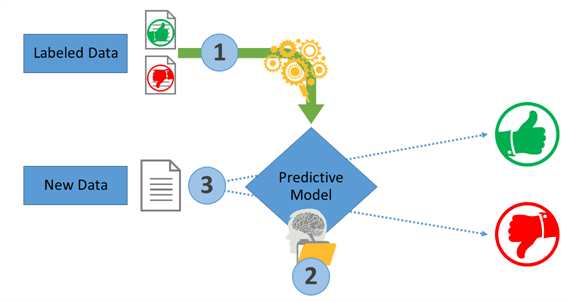
\includegraphics[width=0.6\textwidth]{ml_process_diagram.png}
  	\caption{Diagrama simple del modelo del proyecto.}
  	\end{center}
\end{figure}

\section{Desarrollo}
\subsection{Cliente}
Se utilizará como hardware una \textit{RaspberryPi 3B+} con sistema operativo \textit{Raspbian Stretch}.

\subsection{Servidor}
El hardware será una PC con sistema operativo \textit{Linux Ubuntu 18.04.4 LTS}.

\subsection{Conexión}
Ambas dispositivos estarán conectados a través de cable de red \textit{Fast Ethernet} para simular una red de internet.

\subsection{Funcionamiento general del algoritmo}
El cliente siempre está corriendo esperando conexiones de servidores TCP o UDP. Una vez que llega una conexión posee un \texttt{handler} que se encarga de la misma según su tipo.

En cambio el servidor sólo inicia conexiones una vez que el usuario ingresa los comandos correspondientes.

\subsubsection{\texttt{login()}}
Se pensó en utilizar \textit{hashes} para almacenamiento del \texttt{userpass}, debido a que es la forma que usualmente se guardan las contraseñas.

\begin{lstlisting}
unsigned int string_hash(void *string){
   /* This is the djb2 string hash function */

   unsigned int result = 5381;
   unsigned char *p;

   p = (unsigned char *) string;

   while (*p != '\0') {
	   result = (result << 5) + result + *p;
	   ++p;
   }

   return result;
}
\end{lstlisting}

De esta forma se guardo en variables \texttt{long unsigned int} la contraseña del \texttt{login()}, además se validaron los requerimientos solicitados como cantidad de intentos.

Además se aprovechó esta funcionalidad para sustituir a \texttt{strcmp()} ya que comparando las variables en un \texttt{switch} fácilmente se podían distinguir los comandos ingresados por el usuario.

\subsubsection{\texttt{update firmware.bin}}
Se establece una conexión TCP entre cliente y servidor para la transferencia del archivo. Una vez completada, el cliente se reinicia.

En el cliente fue creado un servicio que corre un \textit{script} que al iniciar el sistema se encarga de verificar si existe un nuevo \textit{bin}, en caso que exista se borra el anterior, se cambia el nombre, se actualiza la versión del \textit{firmware} en un archivo de texto, se le dan permisos de ejecución (\texttt{chmod()}) y se corre nuevamente.

\subsubsection{\texttt{start scanning}}
Se establece una conexión TCP entre el cliente y servidor donde se realiza la transferencia de la imagen, luego se cierra el socket.

\subsubsection{\texttt{obtener telemetria}}
El servidor crea un socket UDP para la conexión. Una vez que el cliente es contactado, envía a través de mensajes UDP los datos requeridos. El servidor se encarga de mostrarlos en consola para el usuario.

\subsection{\texttt{Makefile}}
Se utilizó una cantidad de tiempo considerable en la creación de un archivo \texttt{Makefile} bien configurado para las diferentes pruebas a las que se sometió el sistema puedan ser ejecutadas con rapidez.

\subsubsection{Organización de carpetas}
Se optó por que cada carpeta del proyecto tuviera un tipo de archivo para mejorar la organización.
Entonces en cada carpeta se guardó:
\begin{itemize}
	\item \texttt{bin}: archivos binarios.
	\item \texttt{src}: código fuente y archivos \textit{.o}.
	\item \texttt{include}: \textit{headers}.
\end{itemize}

\subsubsection{Compilación cruzada}
Al principio todo el desarrollo se hizo internamente en una PC, una vez finalizado esto se tenía que migrar al dispositivo cliente.

Sin embargo, para cumplir con los requerimientos de actualización de \textit{firmware} era necesario realizar compilación cruzada, que se define como el acto de compilar código para un sistema informático (a menudo conocido como el objetivo) en un sistema diferente, llamado host.

Fue necesario descargar el \textit{toolkit ARM RaspberryPi} y realizar varias pruebas hasta que se logró su correcto funcionamiento. Esto puede ser revisado en el \texttt{Makefile}.

\section{Conclusión}
Si bien las consignas estaban claras y el desarrollo estaba estructurado algunos pasos tomaron un tiempo considerable, sumado a los problemas que surgieron del ensamblaje final de cada uno de ellos. 

Pero fueron adquiridos conocimientos valiosos como una correcta estructura del proyecto para que el código fuente sea mantenible, además de la documentación del mismo. También se usó \textit{Git} de manera local para los repositorios para la implementación de nuevas \textit{features} a través de ramas.

En síntesis a pesar de ser extenso el proyecto se obtuvieron habilidades en diversas herramientas que serán de utilidad en el futuro maximizando recursos y tiempo.

\clearpage
%\bibliographystyle{ieeetr}
%\\bibliographystyle{unsrtnat}
%\\bibliography{mybib}

\end{document}
